\subsection{Observation}
As a first step, this elaboration provides for the test results of the observation of the test runs. These observations were carried out entirely subjectively and provide information about the reactions of the test candidates when dealing with the two systems. \\
In every other test run, participants took a very long time to reach the home page. This shows that the distraction page works well. After the test run, participants indicated in the feedback session that they would move faster if they did not know they were being tested. Overall, participants who took a long time on the home page stopped reading after a while and immediately scrolled to the top of the page to get to the data table. There were no differences in interaction between the SDS testing system and the normal system. \\
As with the long distraction, participants show a pattern of quickly finding the "Add +" button to add a new entry in both applications. As with the long distraction, participants show the pattern of quickly finding the "Add" button in both applications to add a new entry. Without any response to the second view, participants continue adding data to the form. Observation shows that there is one more entry in the normal application than in the \ac{SDS} application, which is quickly cycled through. But the overall notes show that they were relatively even in their cycle time. \\
Summarizing the observations when adding the data to the table, it seems that entering the data into the normal system was faster. Users quickly enter the data into the form and submit the form immediately. None of the participants ever asked for values for the status because the field was left open as a text box instead of offering a drop-down list. In comparison, two participants in the \ac{SDS} implementation application ask for preset values for status on the form. Of course, this could also be related to bad luck in the selection of participants. \\
All in all, the observations of the test runs show no decisive differences between the two systems. One interaction that stood out in both applications was the tryout pattern. Instead of reading through the text or even the navigation bar elements, users wildly click on any interaction element they find in the view. This resulted in a quick run through the test application, but shows that \ac{SaaS} products should be intuitive to use.

\subsection{Measurements}
From the more subjective measurements to the objective measurements of the time required to complete the test. These measurements can confirm the subjective observations made earlier. Using the measurement points presented in Chapter \ref{text_case}, it is possible to analyze the data collected. If we take the duration between two measurement points, we obtain three time slots. 
\begin{enumerate}
    \item \textbf{Find data table}: Starting the test - see data table
    \item \textbf{Find add button}: See data table - see data add form
    \item \textbf{Add data to table}: See data add forme - submit data add form
\end{enumerate}
With the help of the measurements, it is possible to draw diagrams to understand the collected data better. One problem encountered when looking at the data is that the total duration of each run varies from run to run. A transformation with the collected data ensures that all results are comparable. In detail, the transformation calculates each duration slot relative to the total duration. All sections together result in a total percentage of 100\%. \\

With the prerequisites explained, it's time to look at the data. Starting with the measurements of the test runs on the application without \ac{SDS}.\\

\begin{figure}[htbp]
    \centerline{
    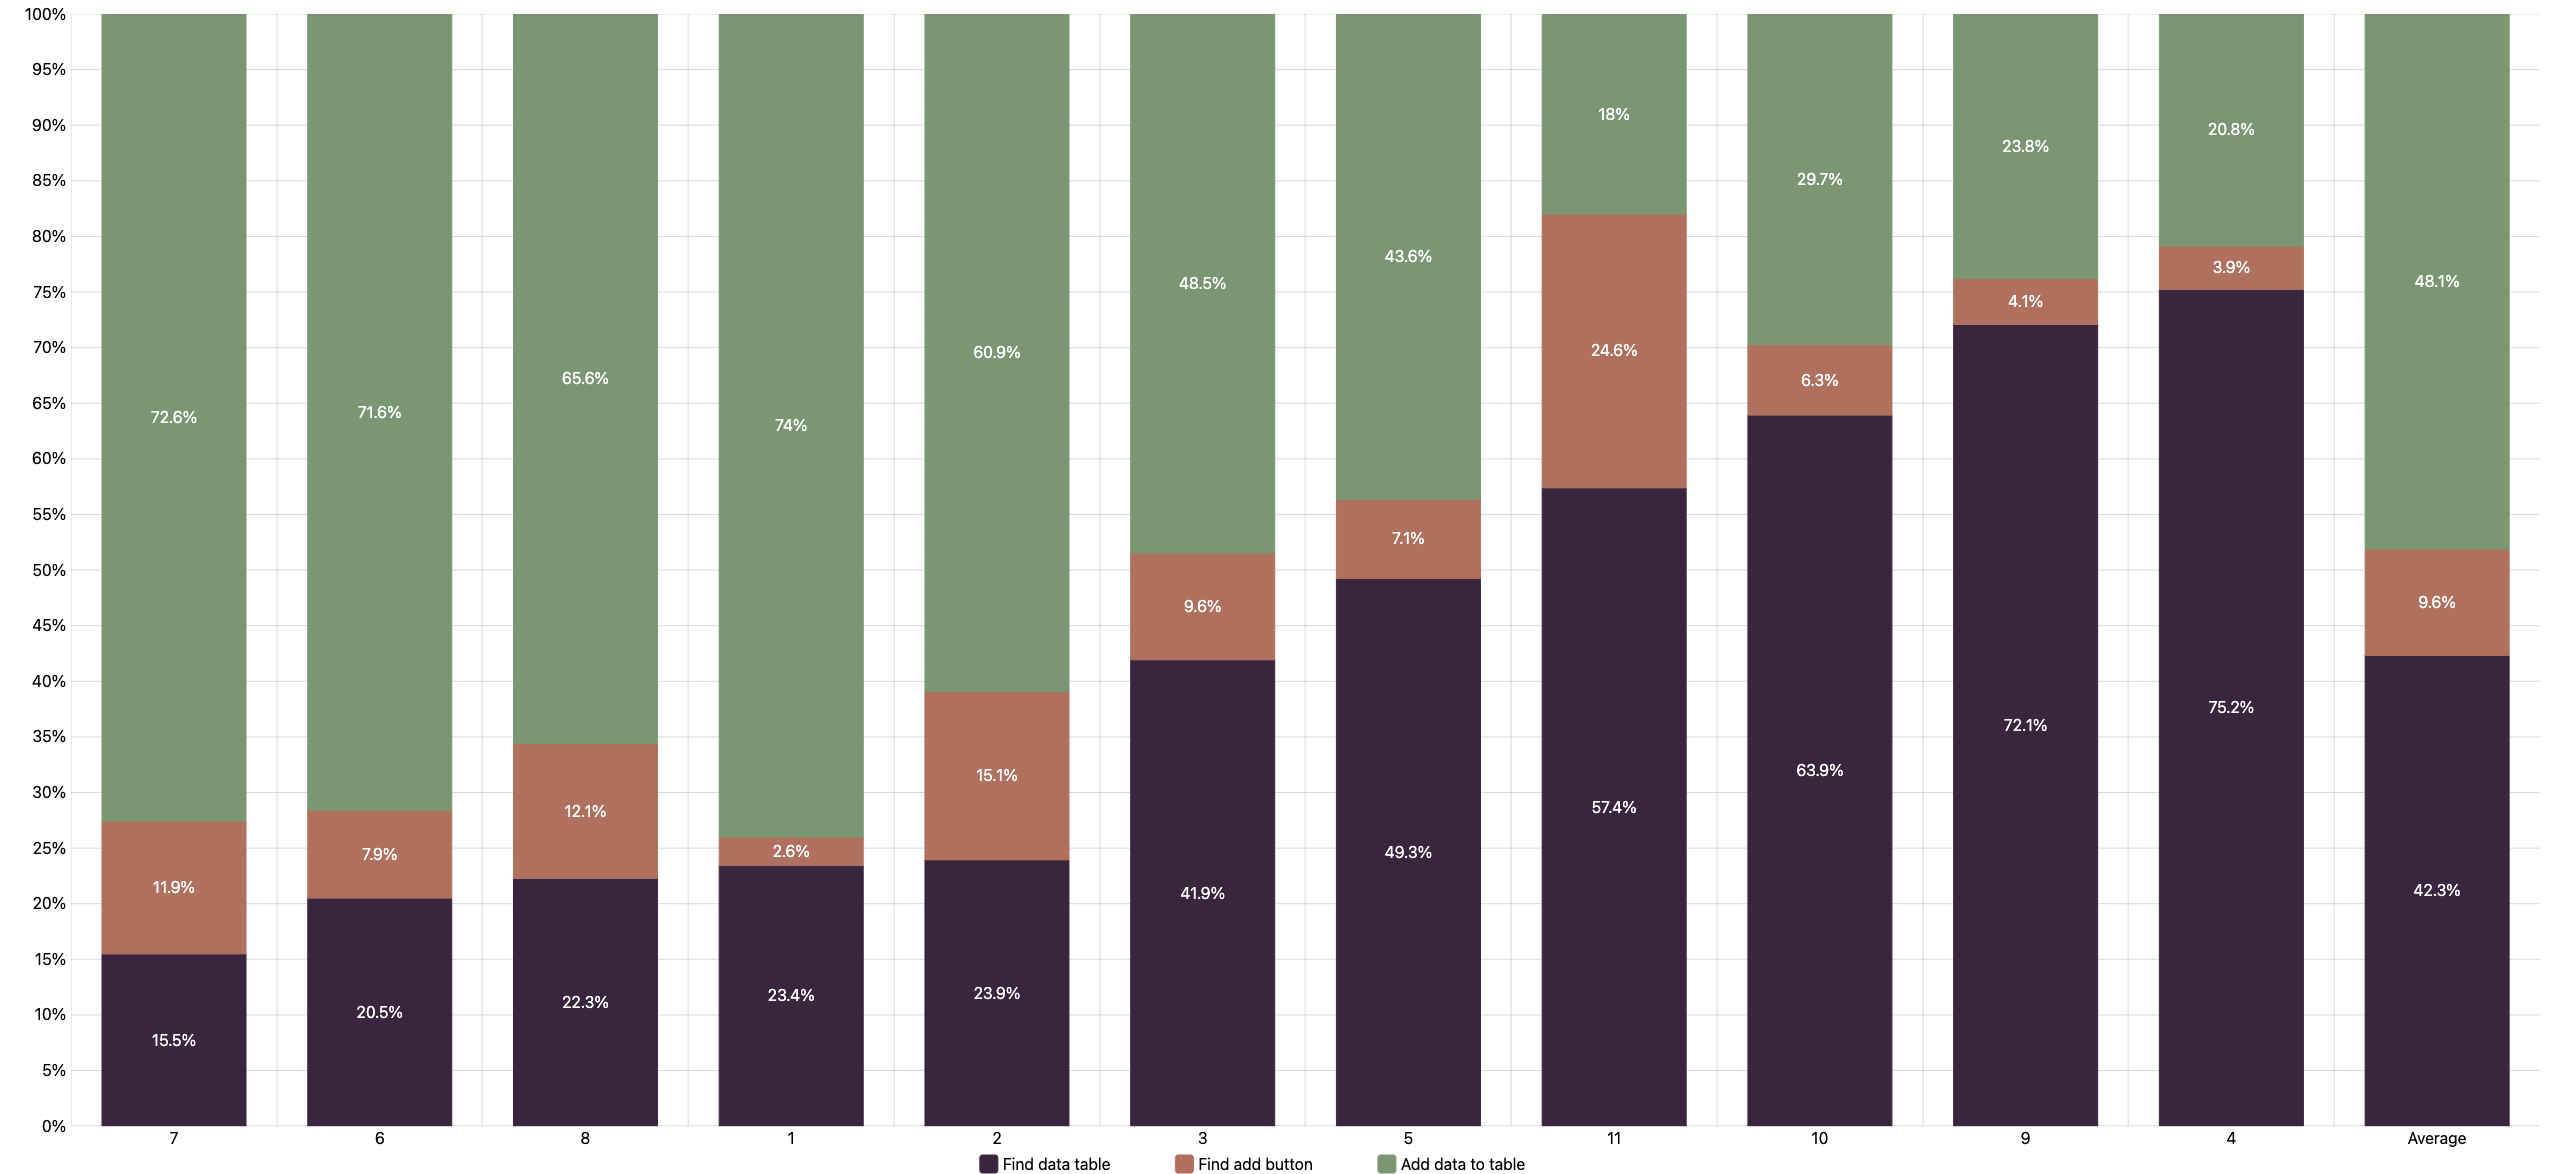
\includegraphics[width=\linewidth]{images/normal_test_data_chart.png}}
\caption{Chart of normal test data}
\label{test_data_normal}
\end{figure}
Looking at the chart in Figure \ref{test_data_normal}, the data confirms the point made in the observations. The chart is sorted by the time it took to find the data table. The first five columns show runs that were completed very quickly. As a result, data entry takes a relatively long time since typing slows down the user. A look at the end of the chart shows the long runs with a longer time on the home page. \\
The last column of the chart shows the average of all datasets combined. Once again, it's important to note that the average time spent on the distribution of finding the data table and adding data through the form is about the same. \\
The only breakout from the schema is test run 11. In this run, the relative number shows that finding the "Add +" button, i.e. showing the data table, took longer than adding the data. A look at the data shows that this was one of the longer test runs of the data set, lasting almost two minutes. Which is probably an indicator that the test user either interacted cautiously with the test application or had trouble navigating.\\
The conclusion of the data chart is that there are no surprises in the test runs for the test application without SDS. It generally confirms the previously reported observation.\\

As a next step, the elaboration deals with the results of the test run of the application with implemented SDS. Expecting to see roughly the same distribution pattern of test data.  As in Figure \ref{test_data_normal}, this chart shows the relative time windows calculated using the total time required for each run. \\

\begin{figure}[htbp]
    \centerline{
    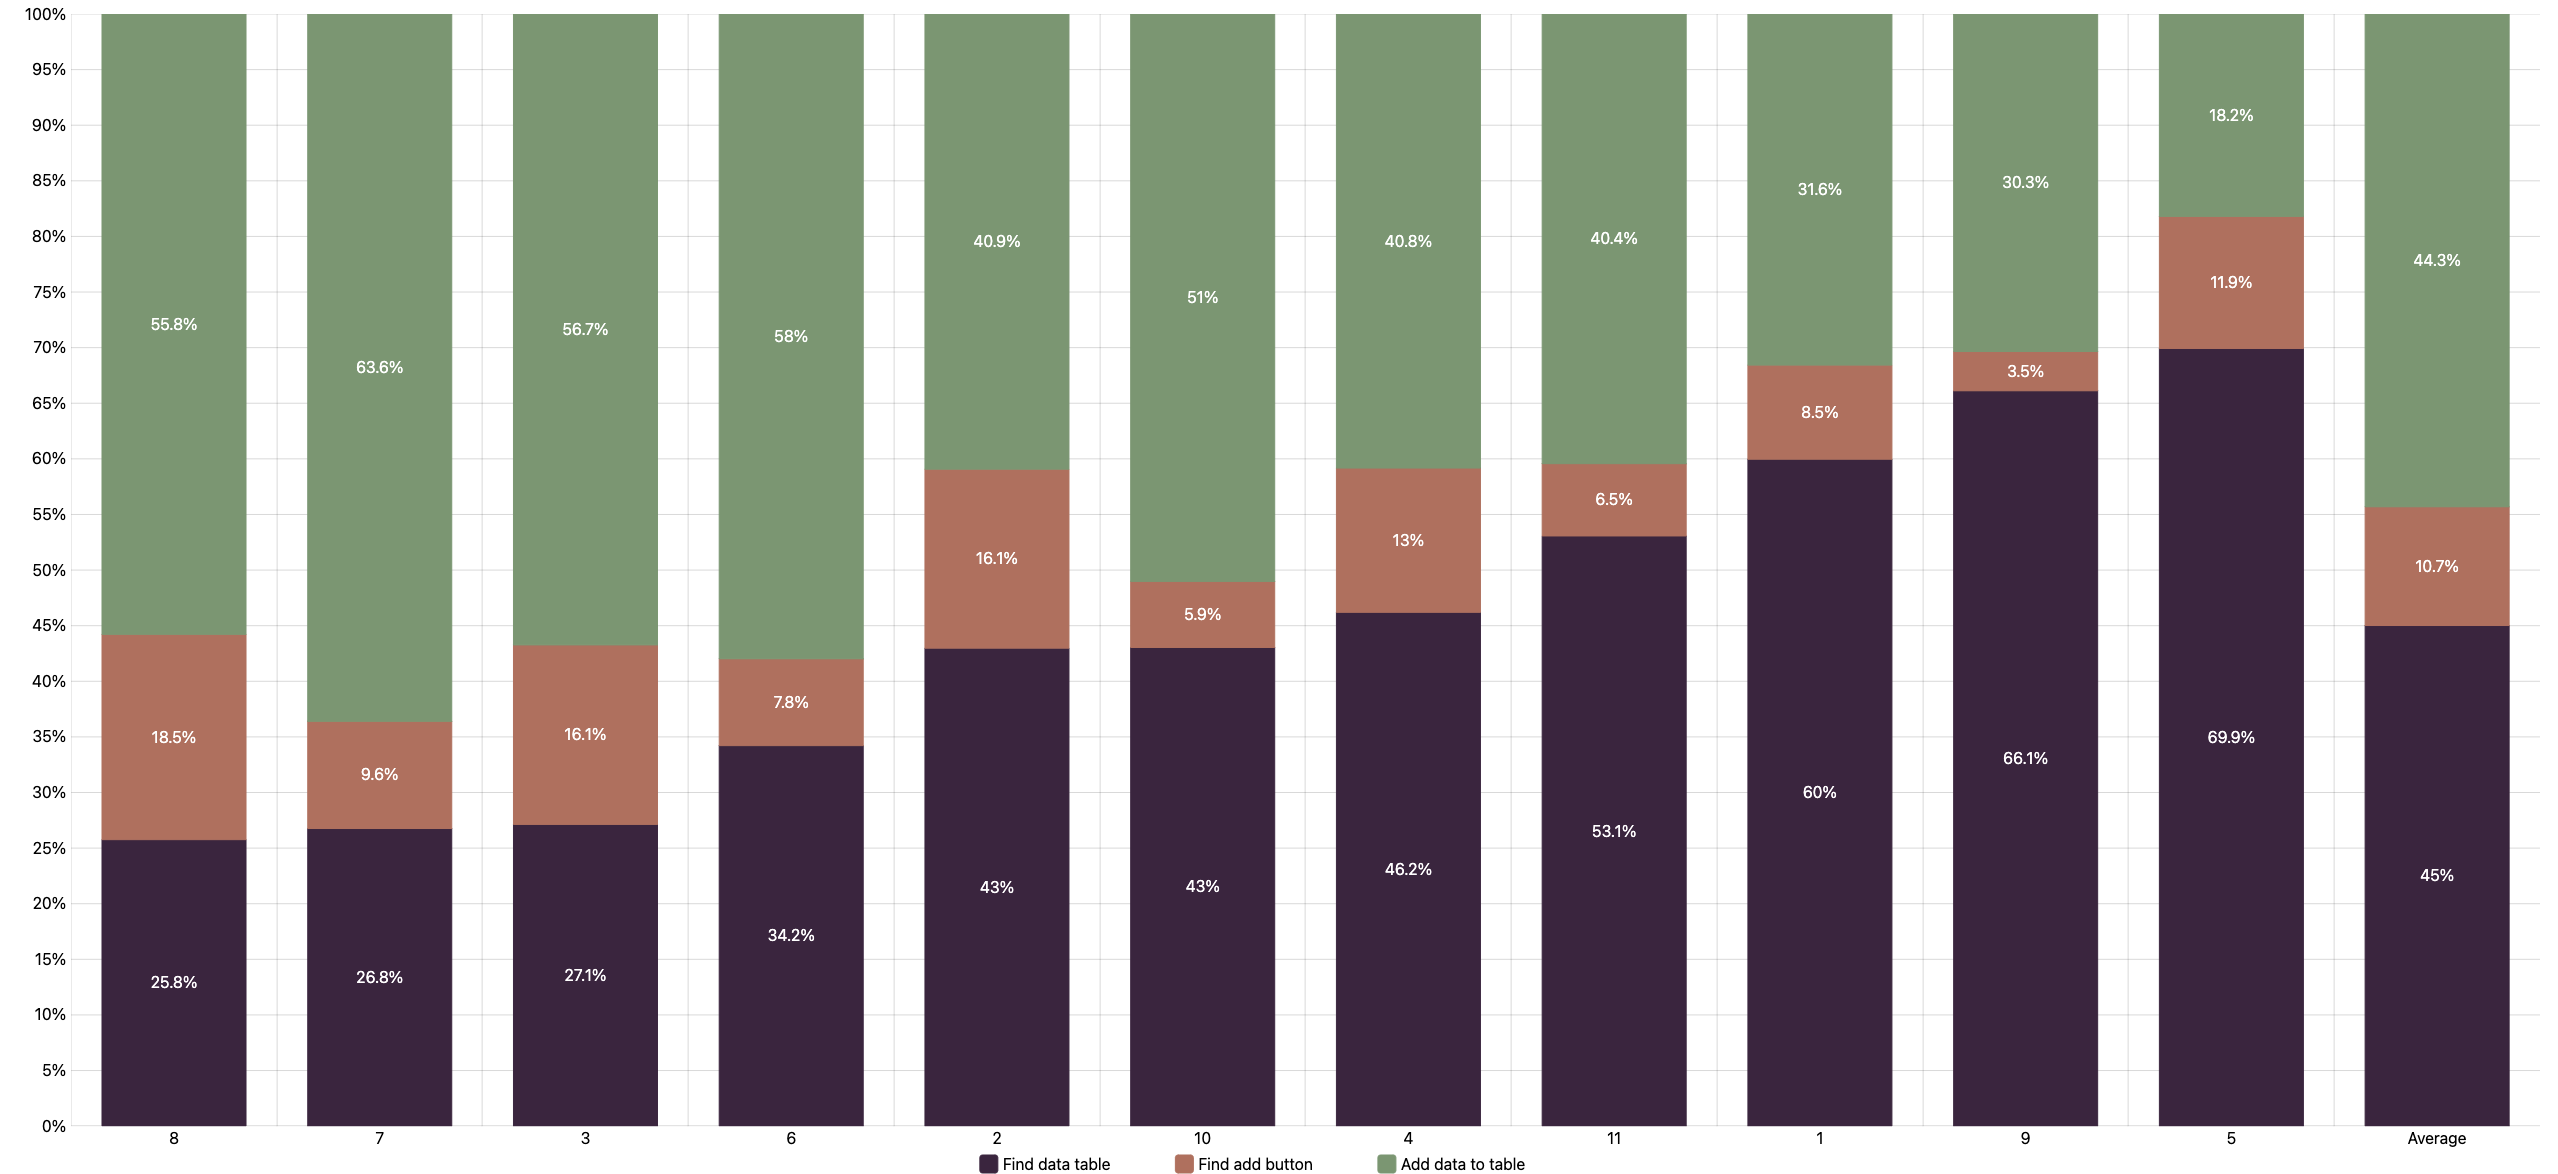
\includegraphics[width=\linewidth]{images/sds_test_data_chart.png}}
\caption{Chart of \ac{SDS} test data}
\label{test_data_sds}
\end{figure}
At first glance, the chart in Figure \ref{test_data_sds} shows the same pattern as the normal test data chart. But in closer comparison to the normal data chart (Figure \ref{test_data_normal}), the distribution of the datasets is smoother. This indicates a more even distribution of the time spent on the different time windows. \\
A look at the average column at the bottom of the chart shows roughly the same distribution of values as the normal data. This means that finding the table of data takes, on average, the same amount of time as entering data into the form. So on average there is no difference to the test application without \ac{SDS}. \\
Looking at breakouts as previously seen on the test device, no test point can be found. The only interesting thing is that in three test runs, the search time for the "Add +" button accounted for over 15\% of the total time. A look at test runs 8, 3, and 2 in Figure \ref{test_data_sds} shows that these test runs are rather short overall. Therefore, a 4-second mouse movement on the button ends in a distribution of 15\% if the total run takes only 30 seconds. However, this is not unusual user behavior in the test application.\\
Summarizing the analysis of the data chart from the test runs of SDS data, the chart shows a smoother curve which could indicate a broader group of test users. Because every user is different when using a tool. In general, the chart shows the same usage patterns as in the normal test data. \\

In order to have comparable test data within the test sets, it was necessary to reduce the data to percentage values. There is no comparison between the two test sets. To do this, the last chart takes both average data points and compares them to each other. \\

\begin{figure}[htbp]
    \centerline{
    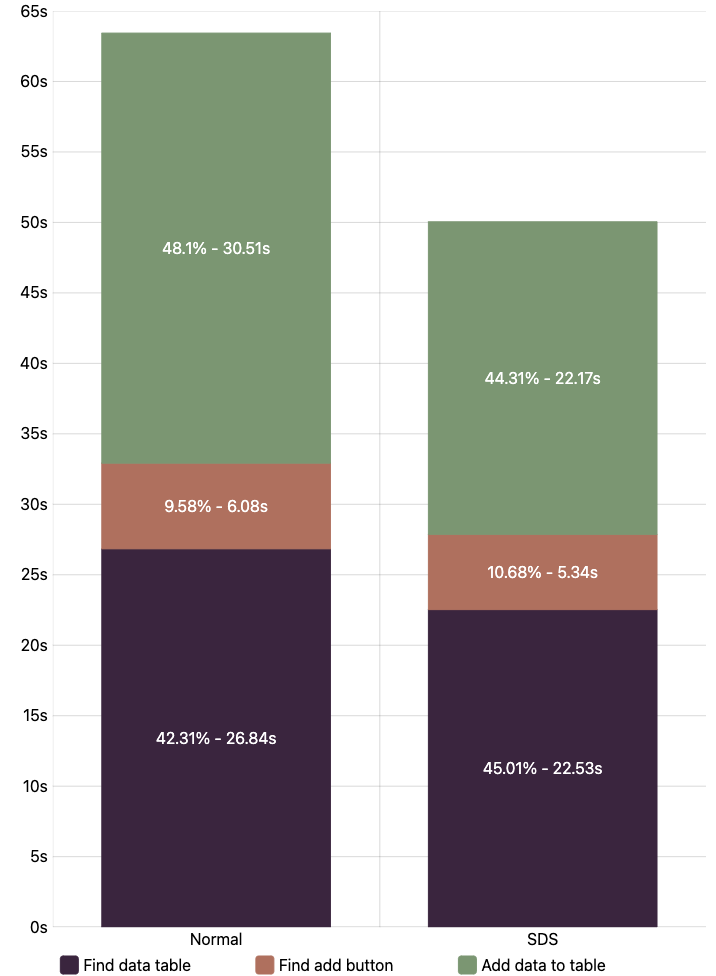
\includegraphics[height=10cm]{images/compare_avarages_test_data_chart.png}}
\caption{Chart of the average test data in comparison}
\label{test_data_avarages_compare}
\end{figure}
In this chart in Figure \ref{test_data_avarages_compare}, the X-axis describes an absolute scale with the total duration of the test runs on average for each test application. And surprisingly, this presentation reveals an interesting insight. \\
As said before, the distribution of the shares of time needed is roughly the same, but in terms of absolute numbers, adding data and finding the table is very different. The chart shows users who tested the application with \ac{SDS} implemented use about 15 seconds less on average than test users of the other system. \\
Finding the data table in the application with the \ac{SDS} takes about 4 seconds less than in the normal test application. This time saving is roughly equivalent to the time it takes to click the "Add +" button to navigate to the third view. But the big difference in the chart shows the bars for adding data to the form. With a difference of 8 seconds less, the test application with \ac{SDS} is significantly better.\\
In contrast to the differences presented before the third category, clicking on the "Add +" does not show any significant differences between the systems. 